\documentclass[aspectratio=169]{beamer}
\usepackage[utf8]{inputenc}
\usepackage{tikz}
\usepackage{listings}
\usepackage{lstautogobble}
\usepackage{wdqs}

\title{Querying Linked Data with SPARQL and the Wikidata Query Service}
\author{Lucas Werkmeister}
\date{2019-12-27}

\usetheme{Rochester}
\beamertemplatenavigationsymbolsempty

\usetikzlibrary{shapes}
\usetikzlibrary{shapes.multipart}

\tikzset{
  % node options
  iri/.style={ellipse,draw},
  literal/.style={rectangle,draw},
  var/.style={ellipse,dashed,draw},
  % path options
  predicate/.style={->,auto},
  predicate bidi/.style={predicate,bend left=5,inner sep=0.25mm},
  % matrix options
  row sep=7mm,
  column sep=15mm,
}

\lstset{language=[wdqs]sparql,autogobble}

\newcommand{\Esszimmer}{\node[iri] (Esszimmer) {Esszimmer};}
\newcommand{\Kueche}{\node[iri] (Kueche) {Küche};}
\newcommand{\thistalk}{\node[iri] (this talk) {this talk};}
\newcommand{\livequerying}{\node[iri] (live querying) {live querying};}
\newcommand{\WikipakaWG}{\node[iri] (WikipakaWG) {WikipakaWG};}
\newcommand{\TagEinsNoon}{\node[literal] (Tag 1 noon) {2019-12-27T\\12:00:00+0100};}
\newcommand{\Congress}{\node[iri] (36C3) {36C3};}
\newcommand{\Klimawahlen}{\node[iri] (Klimawahlen) {Klimawahlen};}
\newcommand{\ChaosWestStage}{\node[iri] (Chaos-West Stage) {Chaos-West\\Stage};}
\newcommand{\ChaosWest}{\node[iri] (Chaos West) {Chaos West};}

\newcommand{\Vlivequerying}{\node[var] (live querying) {\rlap{?talk}\hphantom{live querying}};}
\newcommand{\Vthistalk}{\node[var] (this talk) {\rlap{?talk}\hphantom{this talk}};}
\newcommand{\VEsszimmer}{\node[var] (Esszimmer) {\rlap{?room}\hphantom{Esszimmer}};}

\newcommand{\thistalklivequerying}{\draw[predicate bidi] (this talk) to node {is followed by} (live querying);}
\newcommand{\livequeryingthistalk}{\draw[predicate bidi] (live querying) to node {follows} (this talk);}
\newcommand{\thistalkEsszimmer}{\draw[predicate,bend left] (this talk) to node {happens in} (Esszimmer);}
\newcommand{\livequeryingEsszimmer}{\draw[predicate,swap] (live querying) to node {happens in} (Esszimmer);}
\newcommand{\EsszimmerWikipakaWG}{\draw[predicate,bend left=5] (Esszimmer) to node [pos=.6,inner sep=0] {is part of} (WikipakaWG);}

\begin{document}

\frame{\titlepage}

\begin{frame}[fragile]
  \frametitle{An example graph}
  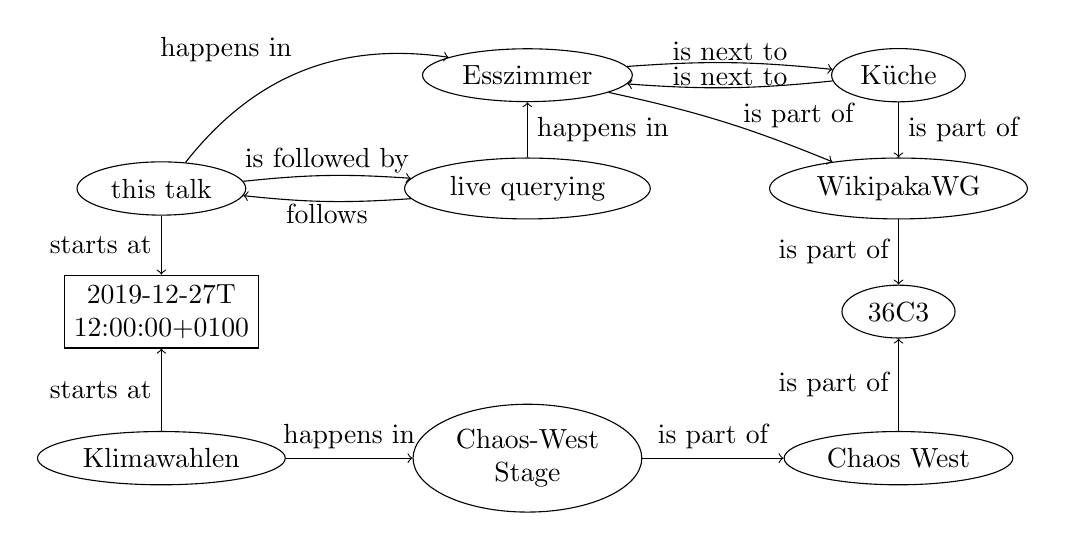
\begin{tikzpicture}[
      every text node part/.style={align=center},
    ]
    \matrix {
      & \Esszimmer & \Kueche \\
      \thistalk & \livequerying & \WikipakaWG \\
      \TagEinsNoon & & \Congress \\
      \Klimawahlen & \ChaosWestStage & \ChaosWest \\
    };
    \thistalklivequerying
    \livequeryingthistalk
    \thistalkEsszimmer
    \livequeryingEsszimmer
    \draw[predicate bidi] (Esszimmer) to node {is next to} (Kueche);
    \draw[predicate bidi,swap] (Kueche) to node {is next to} (Esszimmer);
    \EsszimmerWikipakaWG
    \draw[predicate] (Kueche) to node {is part of} (WikipakaWG);
    \draw[predicate,swap] (WikipakaWG) to node {is part of} (36C3);
    \draw[predicate,swap] (this talk) to node {starts at} (Tag 1 noon);
    \draw[predicate] (Klimawahlen) to node {starts at} (Tag 1 noon);
    \draw[predicate] (Klimawahlen) to node {happens in} (Chaos-West Stage);
    \draw[predicate] (Chaos-West Stage) to node {is part of} (Chaos West);
    \draw[predicate] (Chaos West) to node {is part of} (36C3);
  \end{tikzpicture}
\end{frame}

\begin{frame}[fragile]
  \frametitle{Example questions}
  Which talk follows this one?

  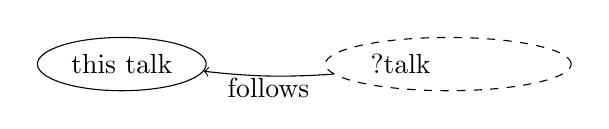
\begin{tikzpicture}
    \matrix {
      \thistalk & \Vlivequerying \\
    };
    \livequeryingthistalk
  \end{tikzpicture}

  Matching triple:

  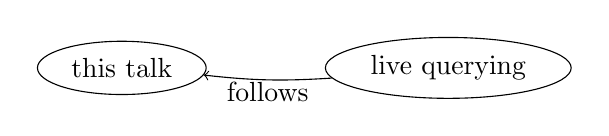
\begin{tikzpicture}
    \matrix {
      \thistalk & \livequerying \\
    };
    \livequeryingthistalk
  \end{tikzpicture}
\end{frame}

\begin{frame}[fragile]
  \frametitle{Example questions}
  Same question, phrased differently:
  Which talk is this one followed by?
  This talk is followed by which one?

  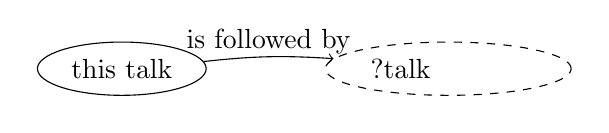
\begin{tikzpicture}
    \matrix {
      \thistalk & \Vlivequerying \\
    };
    \thistalklivequerying
  \end{tikzpicture}

  Matching triple:

  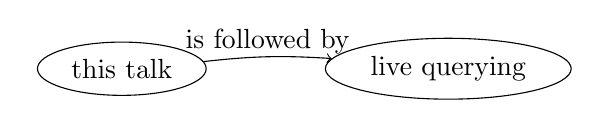
\begin{tikzpicture}
    \matrix {
      \thistalk & \livequerying \\
    };
    \thistalklivequerying
  \end{tikzpicture}
\end{frame}

\begin{frame}[fragile]
  \frametitle{Example questions}
  Which talk happens in Esszimmer?

  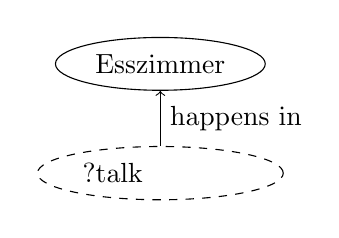
\begin{tikzpicture}
    \matrix {
      \Esszimmer \\
      \Vlivequerying \\
    };
    \livequeryingEsszimmer
  \end{tikzpicture}

  Matching triples:

  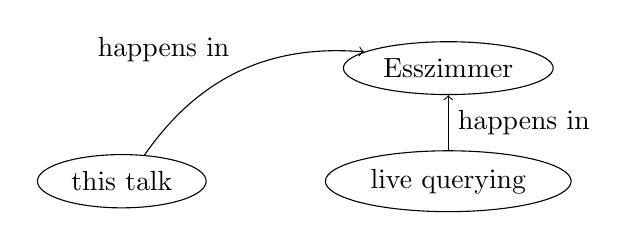
\begin{tikzpicture}
    \matrix {
      & \Esszimmer \\
      \thistalk & \livequerying \\
    };
    \thistalkEsszimmer
    \livequeryingEsszimmer
  \end{tikzpicture}
\end{frame}

\begin{frame}[fragile]
  \frametitle{Example questions}
  Which talks happen in the WikipakaWG?
  That is, which talks happen in a room that’s part of the WikipakaWG?

  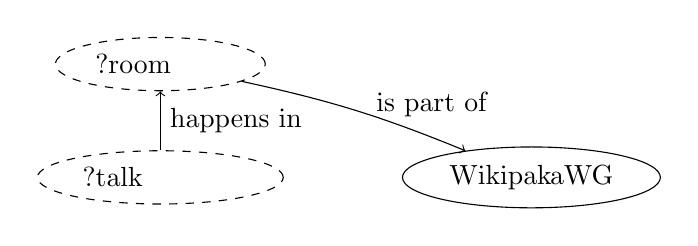
\begin{tikzpicture}
    \matrix {
      \VEsszimmer & \\
      \Vlivequerying & \WikipakaWG \\
    };
    \livequeryingEsszimmer
    \EsszimmerWikipakaWG
  \end{tikzpicture}

  Matching triples:

  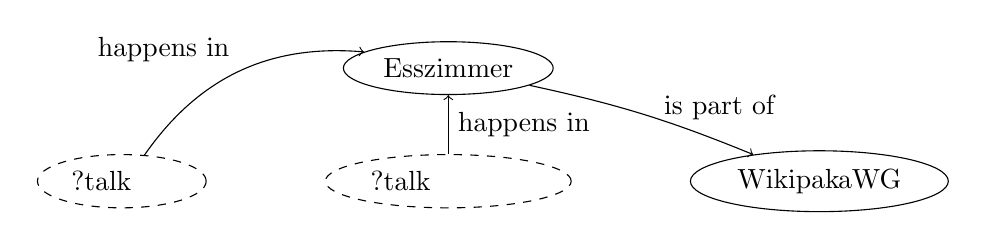
\begin{tikzpicture}
    \matrix {
      & \Esszimmer & \\
      \Vthistalk & \Vlivequerying & \WikipakaWG \\
    };
    \thistalkEsszimmer
    \livequeryingEsszimmer
    \EsszimmerWikipakaWG
  \end{tikzpicture}
\end{frame}

\begin{frame}[fragile]
  \frametitle{SPARQL}
  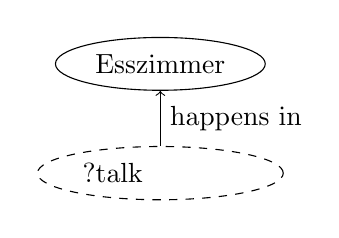
\begin{tikzpicture}
    \matrix {
      \Esszimmer \\
      \Vlivequerying \\
    };
    \livequeryingEsszimmer
  \end{tikzpicture}

  might translate into:

  \begin{lstlisting}
    SELECT * WHERE {
      ?talk 36c3:happensIn 36c3:Esszimmer.
    }
  \end{lstlisting}

  The \lstinline{36c3:} \emph{prefix} clarifies which Esszimmer we’re talking about.
\end{frame}

\begin{frame}[fragile]
  \frametitle{SPARQL}
  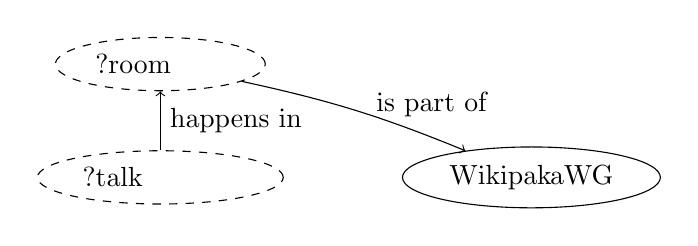
\begin{tikzpicture}
    \matrix {
      \VEsszimmer & \\
      \Vlivequerying & \WikipakaWG \\
    };
    \livequeryingEsszimmer
    \EsszimmerWikipakaWG
  \end{tikzpicture}

  might translate into:

  \begin{lstlisting}
    SELECT * WHERE {
      ?talk 36c3:happensIn ?room.
      ?room 36c3:isPartOf 36c3:WikipakaWG.
    }
  \end{lstlisting}
\end{frame}

\begin{frame}[fragile]
  \frametitle{SPARQL}
  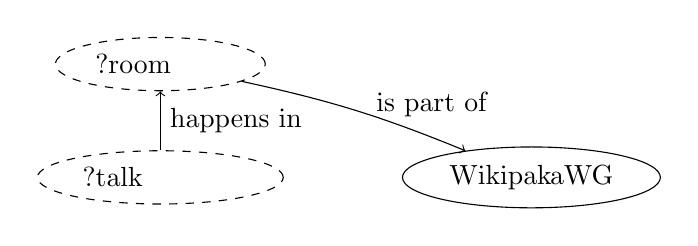
\begin{tikzpicture}
    \matrix {
      \VEsszimmer & \\
      \Vlivequerying & \WikipakaWG \\
    };
    \livequeryingEsszimmer
    \EsszimmerWikipakaWG
  \end{tikzpicture}

  might also translate into:

  \begin{lstlisting}
    SELECT ?talk WHERE {
      ?talk 36c3:happensIn [
        schema:isPartOf 36c3:WikipakaWG
      ].
    }
  \end{lstlisting}
\end{frame}

\end{document}
